\chapter{El Problema}


\section{Introducción}

En esta sección buscaremos dar una descripción mas detallada, tanto del problema a resolver, como así también de cada una de las soluciones adoptas durante el desarrollo del mismo.
Recordemos que el objetivo es desarrollar un agente inteligente, que a partir de un capital inicial, sea capaz de realizar compras y ventas de un activo dentro de un mercado financiero. El agente no poseerá ningún conocimiento previo acerca del funcionamiento del mercado, ni de la empresa sobre la que opera, ni ningun otro tipo de información. Solo conocerá el precio actual de la acción, y su evolución durante los días previos, junto un conjunto de indicadores bursátiles. 

\subsection{Deep reinforcement learning}

El agente va a interactuar con un simulador de un mercado bursátil, esta interacción se llevará a cabo siguiendo una serie de acciones, observaciones y recompensas.
Cada interacción será llevada a cabo en episodios que tendrán una duración de m días

\begin{wrapfigure}{r}{0.5\textwidth}
	\begin{center}
	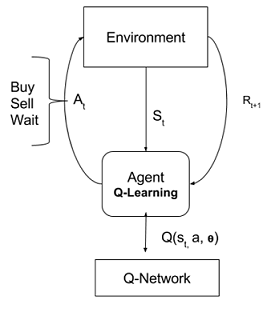
\includegraphics{imagenes/deepRLOverview.png}
	\end{center}
	\caption{Reinforcement Learning Architecture Overview.}
\end{wrapfigure}


En cada instante t, el agente tendrá que seleccionar una acción at  de un conjunto válido de acciones A = {$a_1$, $a_2$, …, $a_n$}. La acción será pasada al entorno, el cual modificará su estado interno y como respuesta a esta interacción el agente recibirá una recompensa (reward), el cual será calculado por el entorno. El entorno será estocástico, es decir, su comportamiento será no determinístico. Cada uno de los estados contendrá información relevante sobre el papel, como el precio, el volumen, y diferentes indicadores bursátiles, como medias móviles, medias móviles exponenciales, etc.

